% Options for packages loaded elsewhere
\PassOptionsToPackage{unicode}{hyperref}
\PassOptionsToPackage{hyphens}{url}
%
\documentclass[
]{article}
\usepackage{lmodern}
\usepackage{amssymb,amsmath}
\usepackage{ifxetex,ifluatex}
\ifnum 0\ifxetex 1\fi\ifluatex 1\fi=0 % if pdftex
  \usepackage[T1]{fontenc}
  \usepackage[utf8]{inputenc}
  \usepackage{textcomp} % provide euro and other symbols
\else % if luatex or xetex
  \usepackage{unicode-math}
  \defaultfontfeatures{Scale=MatchLowercase}
  \defaultfontfeatures[\rmfamily]{Ligatures=TeX,Scale=1}
\fi
% Use upquote if available, for straight quotes in verbatim environments
\IfFileExists{upquote.sty}{\usepackage{upquote}}{}
\IfFileExists{microtype.sty}{% use microtype if available
  \usepackage[]{microtype}
  \UseMicrotypeSet[protrusion]{basicmath} % disable protrusion for tt fonts
}{}
\makeatletter
\@ifundefined{KOMAClassName}{% if non-KOMA class
  \IfFileExists{parskip.sty}{%
    \usepackage{parskip}
  }{% else
    \setlength{\parindent}{0pt}
    \setlength{\parskip}{6pt plus 2pt minus 1pt}}
}{% if KOMA class
  \KOMAoptions{parskip=half}}
\makeatother
\usepackage{xcolor}
\IfFileExists{xurl.sty}{\usepackage{xurl}}{} % add URL line breaks if available
\IfFileExists{bookmark.sty}{\usepackage{bookmark}}{\usepackage{hyperref}}
\hypersetup{
  pdftitle={READ.md},
  pdfauthor={Team 9},
  hidelinks,
  pdfcreator={LaTeX via pandoc}}
\urlstyle{same} % disable monospaced font for URLs
\usepackage[margin=1in]{geometry}
\usepackage{longtable,booktabs}
% Correct order of tables after \paragraph or \subparagraph
\usepackage{etoolbox}
\makeatletter
\patchcmd\longtable{\par}{\if@noskipsec\mbox{}\fi\par}{}{}
\makeatother
% Allow footnotes in longtable head/foot
\IfFileExists{footnotehyper.sty}{\usepackage{footnotehyper}}{\usepackage{footnote}}
\makesavenoteenv{longtable}
\usepackage{graphicx,grffile}
\makeatletter
\def\maxwidth{\ifdim\Gin@nat@width>\linewidth\linewidth\else\Gin@nat@width\fi}
\def\maxheight{\ifdim\Gin@nat@height>\textheight\textheight\else\Gin@nat@height\fi}
\makeatother
% Scale images if necessary, so that they will not overflow the page
% margins by default, and it is still possible to overwrite the defaults
% using explicit options in \includegraphics[width, height, ...]{}
\setkeys{Gin}{width=\maxwidth,height=\maxheight,keepaspectratio}
% Set default figure placement to htbp
\makeatletter
\def\fps@figure{htbp}
\makeatother
\setlength{\emergencystretch}{3em} % prevent overfull lines
\providecommand{\tightlist}{%
  \setlength{\itemsep}{0pt}\setlength{\parskip}{0pt}}
\setcounter{secnumdepth}{-\maxdimen} % remove section numbering

\title{READ.md}
\author{Team 9}
\date{5/4/2021}

\begin{document}
\maketitle

\hypertarget{ux3b5ux3b9ux3c3ux3b1ux3b3ux3c9ux3b3ux3ae}{%
\subsection{Εισαγωγή}\label{ux3b5ux3b9ux3c3ux3b1ux3b3ux3c9ux3b3ux3ae}}

Ο σκοπός αυτού του έγγραφου είναι να περιγράψει το πεδίο ορισμού, τις
απαιτήσεις λογισμικού και την ανάλυση του συστήματος της εφαρμογής
Project Partners.

\hypertarget{ux3b5ux3bcux3b2ux3adux3bbux3b5ux3b9ux3b1}{%
\subsubsection{Εμβέλεια}\label{ux3b5ux3bcux3b2ux3adux3bbux3b5ux3b9ux3b1}}

\hypertarget{ux3b4ux3c5ux3bdux3b1ux3c4ux3ccux3c4ux3b7ux3c4ux3b5ux3c2-ux3bbux3bfux3b3ux3b9ux3c3ux3bcux3b9ux3baux3bfux3cd}{%
\paragraph{Δυνατότητες
Λογισμικού}\label{ux3b4ux3c5ux3bdux3b1ux3c4ux3ccux3c4ux3b7ux3c4ux3b5ux3c2-ux3bbux3bfux3b3ux3b9ux3c3ux3bcux3b9ux3baux3bfux3cd}}

Αρχικά, το λογισμικό επιτρέπει στους διαχειριστές να προσθέσουν μαθήματα
που έχουν ομαδικές εργασίες. Επίσης, θα δημιουργεί τον λογαριασμό του
φοιτητή, με βάση τον αριθμό μητρώου του και θα αποθηκεύει τα στοιχεία
του. Το σύστημα θα επιτρέπει στον φοιτητή να ενημερώσει τα στοιχεία αυτά
όποτε επιθυμεί, με την προϋπόθεση να υποβάλλει τον κωδικό του. Έπειτα το
σύστημα του παρουσιάζει τα μαθήματα της σχολής, που απαιτούν την
εκπόνηση μίας ομαδικής εργασίας φιλτραρισμένα ανά εξάμηνο. Ο φοιτητής
επιλέγει τα μαθήματα στα οποία αναζητεί ομάδα, το σύστημα αποθηκεύει τις
επιλογές του και ύστερα του εμφανίζει τις διαθέσιμες ομάδες ανά μάθημα.
Στη συνέχεια εάν διαλέξει μία από τις διαθέσιμες ομάδες, το σύστημα
ειδοποιεί τον υπεύθυνο εκείνης της ομάδας και περιμένει έγκριση από
αυτόν, για να πραγματοποιηθεί η εγγραφή του φοιτητή σε αυτή την ομάδα.
Ωστόσο, εάν δεν επιλέξει καμία από τις διαθέσιμες ομάδες, το σύστημα του
δίνει τη δυνατότητα να δημιουργήσει μία δική του, θέτοντας ένα όριο στον
δυνατό αριθμό μελών, στην οποία θα ορίσει αυτός τις δικές του
απαιτήσεις. Μετά την ολοκλήρωση του εξαμήνου, το σύστημα θα δέχεται
ανώνυμες αξιολογήσεις μεταξύ των φοιτητών που συνεργάστηκαν και
αποσυνθέτει τις ομάδες.

\hypertarget{ux3bbux3b5ux3b9ux3c4ux3bfux3c5ux3c1ux3b3ux3afux3b5ux3c2-ux3b5ux3baux3c4ux3ccux3c2-ux3c4ux3c9ux3bd-ux3b4ux3c5ux3bdux3b1ux3c4ux3bfux3c4ux3aeux3c4ux3c9ux3bd-ux3c4ux3bfux3c5-ux3bbux3bfux3b3ux3b9ux3c3ux3bcux3b9ux3baux3bfux3cd}{%
\paragraph{Λειτουργίες εκτός των δυνατοτήτων του
λογισμικού}\label{ux3bbux3b5ux3b9ux3c4ux3bfux3c5ux3c1ux3b3ux3afux3b5ux3c2-ux3b5ux3baux3c4ux3ccux3c2-ux3c4ux3c9ux3bd-ux3b4ux3c5ux3bdux3b1ux3c4ux3bfux3c4ux3aeux3c4ux3c9ux3bd-ux3c4ux3bfux3c5-ux3bbux3bfux3b3ux3b9ux3c3ux3bcux3b9ux3baux3bfux3cd}}

Το λογισμικό δεν επιτρέπει να συνδεθεί ο χρήστης χωρίς να έχει αριθμό
μητρώου, δεν δίνει πρόσβαση στον χρήστη χωρίς σωστή υποβολή του κωδικού
του, δεν επιτρέπει να φτιάξει ο χρήστης πάνω από μια ομάδες στο ίδιο
μάθημα, δεν αφήνει το χρήστη να αξιολογήσει κάποιο συμφοιτητή του αν δεν
έχει συνεργαστεί μαζί του τουλάχιστον μία φορά, δεν δίνει τη δυνατότητα
στον φοιτητή να δει τα στοιχεία επικοινωνίας των ατόμων που δεν είναι
στην ομάδα του, δεν αφήνει τον χρήστη να ενημερώσει τα στοιχεία του εάν
δεν υποβάλλει τον κωδικό του για λόγους εξακρίβωσης, δεν επιτρέπει μία
ομάδα να υπερβεί το μέγιστο αριθμό μελών.

\begin{figure}
\centering
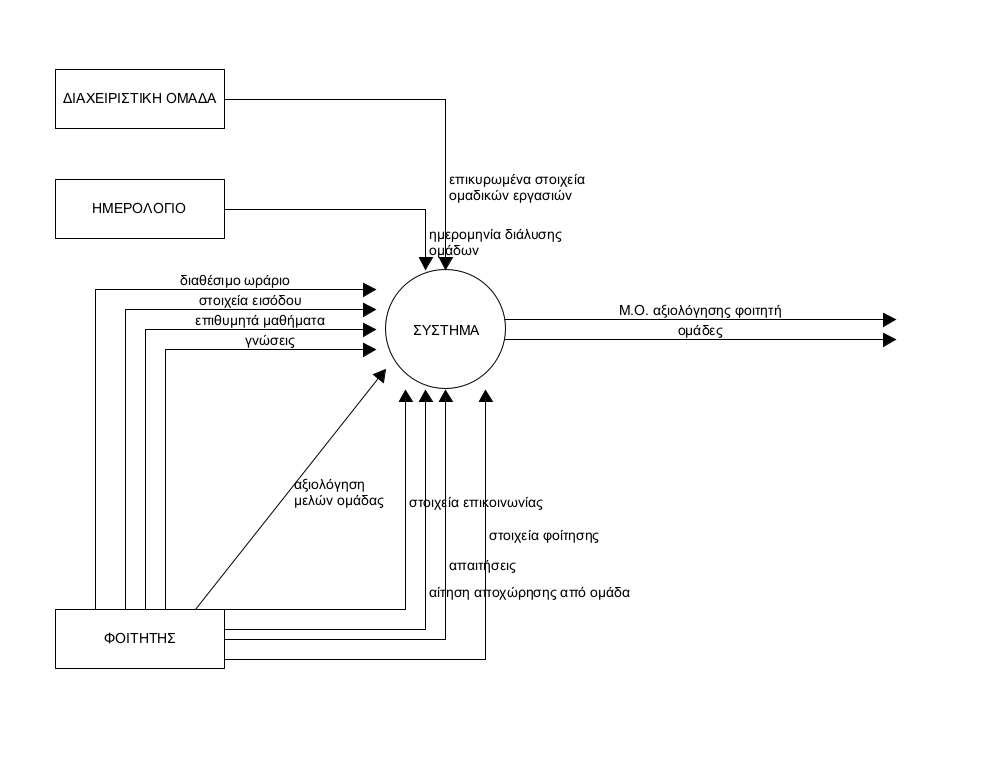
\includegraphics{1.png}
\caption{\emph{Data Flow Diagram}}
\end{figure}

\hypertarget{ux3b1ux3baux3c1ux3ceux3bdux3c5ux3bcux3b1-ux3baux3b1ux3b9-ux3c3ux3c5ux3bdux3c4ux3bfux3bcux3bfux3b3ux3c1ux3b1ux3c6ux3afux3b5ux3c2}{%
\subsubsection{Ακρώνυμα και
Συντομογραφίες}\label{ux3b1ux3baux3c1ux3ceux3bdux3c5ux3bcux3b1-ux3baux3b1ux3b9-ux3c3ux3c5ux3bdux3c4ux3bfux3bcux3bfux3b3ux3c1ux3b1ux3c6ux3afux3b5ux3c2}}

\begin{longtable}[]{@{}ll@{}}
\toprule
\begin{minipage}[b]{0.37\columnwidth}\raggedright
Έννοια\strut
\end{minipage} & \begin{minipage}[b]{0.57\columnwidth}\raggedright
Επεξήγηση\strut
\end{minipage}\tabularnewline
\midrule
\endhead
\begin{minipage}[t]{0.37\columnwidth}\raggedright
Αριθμός Μητρώου\strut
\end{minipage} & \begin{minipage}[t]{0.57\columnwidth}\raggedright
Ο μοναδικός αριθμός που δίνεται σε κάθε φοιτητή κατά την εγγραφή της
σχολής\strut
\end{minipage}\tabularnewline
\begin{minipage}[t]{0.37\columnwidth}\raggedright
Φοιτητής\strut
\end{minipage} & \begin{minipage}[t]{0.57\columnwidth}\raggedright
Ο μαθητής που σπουδάζει και φοιτά στο πανεπιστήμιο\strut
\end{minipage}\tabularnewline
\begin{minipage}[t]{0.37\columnwidth}\raggedright
Ημερολόγιο\strut
\end{minipage} & \begin{minipage}[t]{0.57\columnwidth}\raggedright
Σύστημα που αναγράφει όλες τις ημέρες του έτους\strut
\end{minipage}\tabularnewline
\begin{minipage}[t]{0.37\columnwidth}\raggedright
Διαχειριστική Ομάδα\strut
\end{minipage} & \begin{minipage}[t]{0.57\columnwidth}\raggedright
Η ομάδα που είναι υπεύθυνη για τη διαχείρηση ενός συστήματος\strut
\end{minipage}\tabularnewline
\bottomrule
\end{longtable}

\hypertarget{ux3b5ux3c0ux3b9ux3c3ux3baux3ccux3c0ux3b7ux3c3ux3b7}{%
\subsubsection{Επισκόπηση}\label{ux3b5ux3c0ux3b9ux3c3ux3baux3ccux3c0ux3b7ux3c3ux3b7}}

Στη συνέχεια θα παρουσιαστεί μία γενική εικόνα του συστήματος με τη
χρήση ενός μοντέλου περιπτώσεων χρήσης. Έπειτα θα ακολουθήσουν οι
απαιτήσεις του λογισμικού αλλά και η ανάλυση του συστήματος.

\hypertarget{ux3bcux3bfux3bdux3c4ux3adux3bbux3bf-ux3c0ux3b5ux3c1ux3b9ux3c0ux3c4ux3ceux3c3ux3b5ux3c9ux3bd-ux3c7ux3c1ux3aeux3c3ux3b7ux3c2}{%
\subsubsection{Μοντέλο Περιπτώσεων
Χρήσης}\label{ux3bcux3bfux3bdux3c4ux3adux3bbux3bf-ux3c0ux3b5ux3c1ux3b9ux3c0ux3c4ux3ceux3c3ux3b5ux3c9ux3bd-ux3c7ux3c1ux3aeux3c3ux3b7ux3c2}}

\begin{figure}
\centering
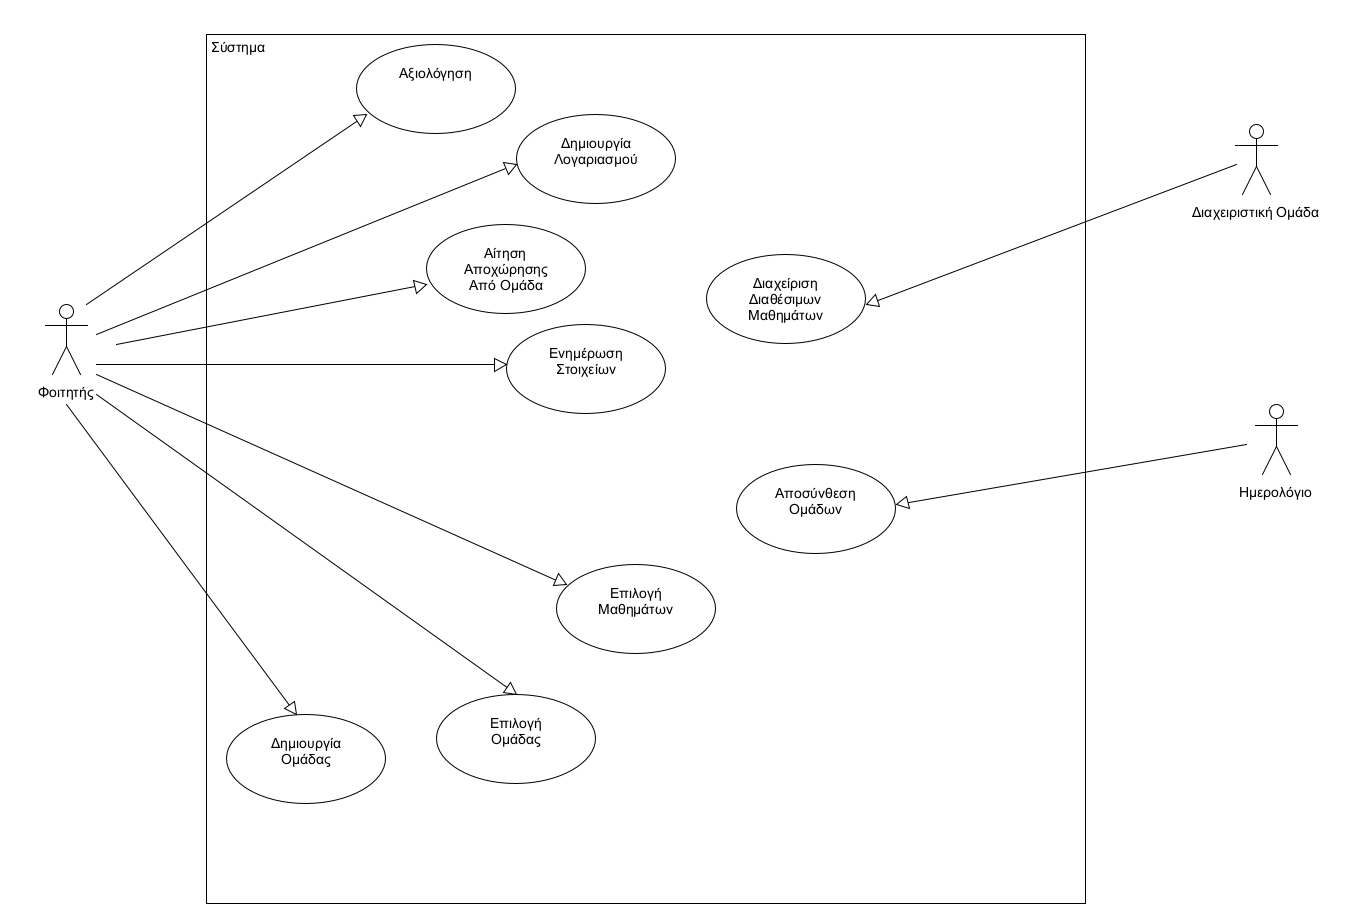
\includegraphics{2.png}
\caption{\emph{Use Case}}
\end{figure}

\begin{longtable}[]{@{}ll@{}}
\toprule
\begin{minipage}[b]{0.35\columnwidth}\raggedright
Περιπτώσεις χρήσης\strut
\end{minipage} & \begin{minipage}[b]{0.59\columnwidth}\raggedright
Ανάλυση Περιπτώσεων Χρήσης\strut
\end{minipage}\tabularnewline
\midrule
\endhead
\begin{minipage}[t]{0.35\columnwidth}\raggedright
\textbf{ΠΧ Δημιουργία Ομάδας}\strut
\end{minipage} & \begin{minipage}[t]{0.59\columnwidth}\raggedright
Ο φοιτητής δημιουργεί μία δική του ομάδα αντί να εγγραφεί σε μία
υπάρχουσα\strut
\end{minipage}\tabularnewline
\begin{minipage}[t]{0.35\columnwidth}\raggedright
\textbf{ΠΧ Επιλογή Ομάδας}\strut
\end{minipage} & \begin{minipage}[t]{0.59\columnwidth}\raggedright
Ο φοιτητής επιλέγει μία υπάρχουσα ομάδα\strut
\end{minipage}\tabularnewline
\begin{minipage}[t]{0.35\columnwidth}\raggedright
\textbf{ΠΧ Επιλογή Μαθημάτων}\strut
\end{minipage} & \begin{minipage}[t]{0.59\columnwidth}\raggedright
Ο φοιτητής επιλέγει τα μαθήματα που θα χρειαστεί ομαδική εργασία το
τρέχον εξάμηνο\strut
\end{minipage}\tabularnewline
\begin{minipage}[t]{0.35\columnwidth}\raggedright
\textbf{ΠΧ Ενημέρωση Στοιχείων}\strut
\end{minipage} & \begin{minipage}[t]{0.59\columnwidth}\raggedright
Ο φοιτητής ενημερώνει τα στοιχεία του λογαριασμού του\strut
\end{minipage}\tabularnewline
\begin{minipage}[t]{0.35\columnwidth}\raggedright
\textbf{ΠΧ Αίτηση Αποχώρησης Από Ομάδα}\strut
\end{minipage} & \begin{minipage}[t]{0.59\columnwidth}\raggedright
Ο φοιτητής αιτείται να αποχωρήσει από μία ομάδα που είναι
εγγεγραμμένος\strut
\end{minipage}\tabularnewline
\begin{minipage}[t]{0.35\columnwidth}\raggedright
\textbf{ΠΧ Δημιουργία Λογαριασμού}\strut
\end{minipage} & \begin{minipage}[t]{0.59\columnwidth}\raggedright
Ο φοιτητής δημιουργεί τον λογαριασμό του\strut
\end{minipage}\tabularnewline
\begin{minipage}[t]{0.35\columnwidth}\raggedright
\textbf{ΠΧ Αξιολόγηση}\strut
\end{minipage} & \begin{minipage}[t]{0.59\columnwidth}\raggedright
Ο φοιτητής αξιολογεί κάποιο συμφοιτητή του με τον οποίο
συνεργάστηκε\strut
\end{minipage}\tabularnewline
\begin{minipage}[t]{0.35\columnwidth}\raggedright
\textbf{ΠΧ Διαχείρηση Διαθέσιμων Μαθημάτων}\strut
\end{minipage} & \begin{minipage}[t]{0.59\columnwidth}\raggedright
Η διαχειριστική ομάδα οργανώνει τα διαθέσιμα μαθήματα του τρέχοντος
εξαμήνου\strut
\end{minipage}\tabularnewline
\begin{minipage}[t]{0.35\columnwidth}\raggedright
\textbf{ΠΧ Αποσύνθεση Ομάδων}\strut
\end{minipage} & \begin{minipage}[t]{0.59\columnwidth}\raggedright
Το ημερολόγιο στην ημερομηνία που υποδείχτηκε ότι τελειώνει το εξάμηνο
αποσυνθέτει τις ομάδες\strut
\end{minipage}\tabularnewline
\bottomrule
\end{longtable}

\end{document}
